\section{Basics of probability}

\subsection{Random Variable, Density}

\begin{mybox}
\begin{definition}
[Random Variable]\label{def:rv}
    Random variable is defined by the Kolmogorov triplet $(\Omega, \mathcal{F}, P)$, where
    \begin{enumerate}
        \item $\Omega$ is the set of all possible outcomes \kir{set of all values of our random variable}
        \item $\mathcal{F}$ is the sigma-algebra (it's a specific set of subsets) defined on $\Omega$ \kir{we would like to ask some questions like "what's the probability that our random variable is less than 5?"; hence we need to reason about subsets of $\Omega$}
        \begin{enumerate}
            \item $\Omega \in \mathcal{F}$ \kir{indeed, we have to reason about the probability of the entire set}
            \item if $A \in \mathcal{F}$ then $\Omega \backslash A \in \mathcal{F}$ \kir{because we want to reason about event $A$ happening and NOT happening}
            \item if $A_i \in \mathcal{F}\,, \; \forall i = 1,2,\ldots$ then $\cup_{i=1}^\infty A_i \in \mathcal{F}$ \kir{because of the additivity of the measure below}
        \end{enumerate}
        \item $P: \mathcal{F} \to [0,1]$ the probability measure \kir{it's a map from subsets to numbers}
        \begin{enumerate}
            \item $P(\Omega) = 1$ \kir{that's quite clear}
            \item $P(\cup_{i=1}^\infty A_i) = \sum_{i=1}^\infty P(A_i)$ for $A_i \in \mathcal{F}\,,\; \forall i$ and $A_i \cap A_j = \varnothing\,,\; \forall i,j$. \kir{indeed, if we consider a union of several non-overlapping events, their probabilities have to add up}
        \end{enumerate}
    \end{enumerate}
\end{definition}
\end{mybox}

The sigma-algebra in this definition carries a lot of the work, because it designs the set of subsets which probability you can measure (input into $P$). 
To understand this, the following two 
\begin{exercise}
    Prove that $\mathcal{F}$ also contains the intersections, i.e. if $A_i \in \mathcal{F}\,, \; \forall i = 1,2,\ldots$ then $\cap_{i=1}^\infty A_i \in \mathcal{F}$.
\end{exercise}
\begin{exercise}
    Construct the Borel sigma-algebra (minimal sigma-algebra containing all the open sets $(a,b), a < b$) on the unit interval $[0,1]$.
\end{exercise}

The definition of the random variable is the central concept of probability theory (formulated by Kolmogorov) and you can't escape it.
This definition is not how people reason about probabilities in practice, though.
It is a distilled concept that serves as a solid foundation to the probability theory and everything that uses it. 
If you would like to know more about it you should read books on Measure theory, Probability theory, Stochastic processes.
Note that this will lead you downwards to the studies of the essence and the atomic ideas (at ``nanoscales'') of probability theory and pure mathematics.
In this course we will go upwards and will construct concepts on top of the probability theory.
For that purpose we will need more visual and intuitive definitions of random variables.

\begin{mybox}
\begin{definition}
[Discrete random variable]\label{def:discrete_rv}    
    We can define discrete random variables in a straightforward way following the definition of the random variable
    \begin{enumerate}
        \item $\Omega$ is a countable set of all outcomes \kir{think about categorical distribution, or a random walk on integers}
        \item $\mathcal{F} = 2^\Omega$ \kir{we can simply choose the set of all subsets, and, in that sense the sigma-algebra definition is not working at its fullest, but, this is not the only possible choice of a sigma-algebra on a finite set}
        \item $P: 2^\Omega \to [0,1]$. For instance, $\forall A \in \mathcal{F}$ it's going to be a simple enumeration $P(A) = \sum_{\omega \in A} P(\omega)$. \kir{hence, we just need to define $P: \Omega \to [0,1]$, and the rest is an accounting job.}
    \end{enumerate}
\end{definition}
\end{mybox}

You can see that in \cref{def:discrete_rv} we barely used the definition of a random variable. 
Indeed, for every outcome $\omega$ in the (countable) set of all outcomes $\Omega$, we can just define a non-negative number $P(\omega) \geq 0$ (we can also exclude all the outcomes $\omega$ for which $P(\omega) = 0$) and then make sure that the total probability sums up to $1$, i.e.
\begin{align}
    P(\Omega) = \sum_{\omega \in \Omega} P(w) = 1\,.
\end{align}
From the perspective of the probability theory, this is great because our definition describes one of the most important use-cases in a meaningful way.
From the practical perspective, the theory doesn't tell us anything new, just gives us a thumbs up. \kir{note that the probability theory for discrete variables in this form existed long before Hilbert and Kolmogorov (mathematical foundation of probability theory was one of the problems proposed by Hilbert in 1900, which was solved by Kolmogorov in 1933)}.

\begin{mybox}
\begin{definition}[Continuous random variable]\label{def:continuous_rv}
    The definition of the random variable shines when we have to meticulously define a new random variable which is a subject of our studies \kir{which is not what usually happens in practice}.
    \begin{enumerate}
        \item $\Omega = \mathbb{R}^n$ \kir{in the course we will consider only the Euclidian space or some simple subset of it.}
        \item $\mathcal{F}$ is the Borel sigma-algebra, i.e. the minimal sigma-algebra containing all the open subsets (i.e. start constructing from $(a,b), a < b$ for $\mathbb{R}$).
        \item $P: \mathcal{F} \to [0,1]$ probability measure is what defines our random variable \kir{in the sense that there are a lot of different random variables with the same $\Omega, \mathcal{F}$ and different $P$}.
    \end{enumerate}
\end{definition}
\end{mybox}

Continuous random variables is the main reason why people still learn/teach/discuss \cref{def:rv}.
It is the rock bottom (of probability theory and everything on top of it) that you hit if you keep asking the question ``why?''.
So far nobody has found cracks in it (doesn't mean there is no any) and we keep on using it and everything works.
However, keeping in mind the sigma-algebras and all the corner cases is not necessary in most of the practical scenarios.
It is simply not the right tool that allows you to solve practical problems.
Much more useful tool in practice is the concept of the probability density.

\begin{mybox}
\begin{definition}[Probability Density Function]\label{def:pdf}
    Consider the random variable $X$ defined as the triplet $(\Omega, \mathcal{F}, P)$, then for any $A \in \mathcal{F}$ we have
    \begin{align}
        \int_{A} dx\; p(x) = P(X \in A)\,,
    \end{align}
    where the integrated (Lebesgue integral) function $p(x)$ is called Probability Density Function (PDF) or simply ``density''.
\end{definition}
\end{mybox}

The probability density function $p(x)$ is not a probability and doesn't tell you anything about any probability until you perform the integration! \kir{you can prove that points also belong to sigma-algebras but their measure is zero, i.e., for $A = \{y\}$ the probability $P(X \in A) = 0$}

The useful way to think about the density is geometric, i.e. think that you can draw any area in the Euclidian space \kir{but not something egregious, which is taken care of by the sigma-algebra} then the density is a magic black box that allows you to calculate the probability that your random variable is going to be in this area.
The density can be visualized in the same way as any function (see \cref{fig:densities_visualization}).

\begin{figure}[t]
    \centering
    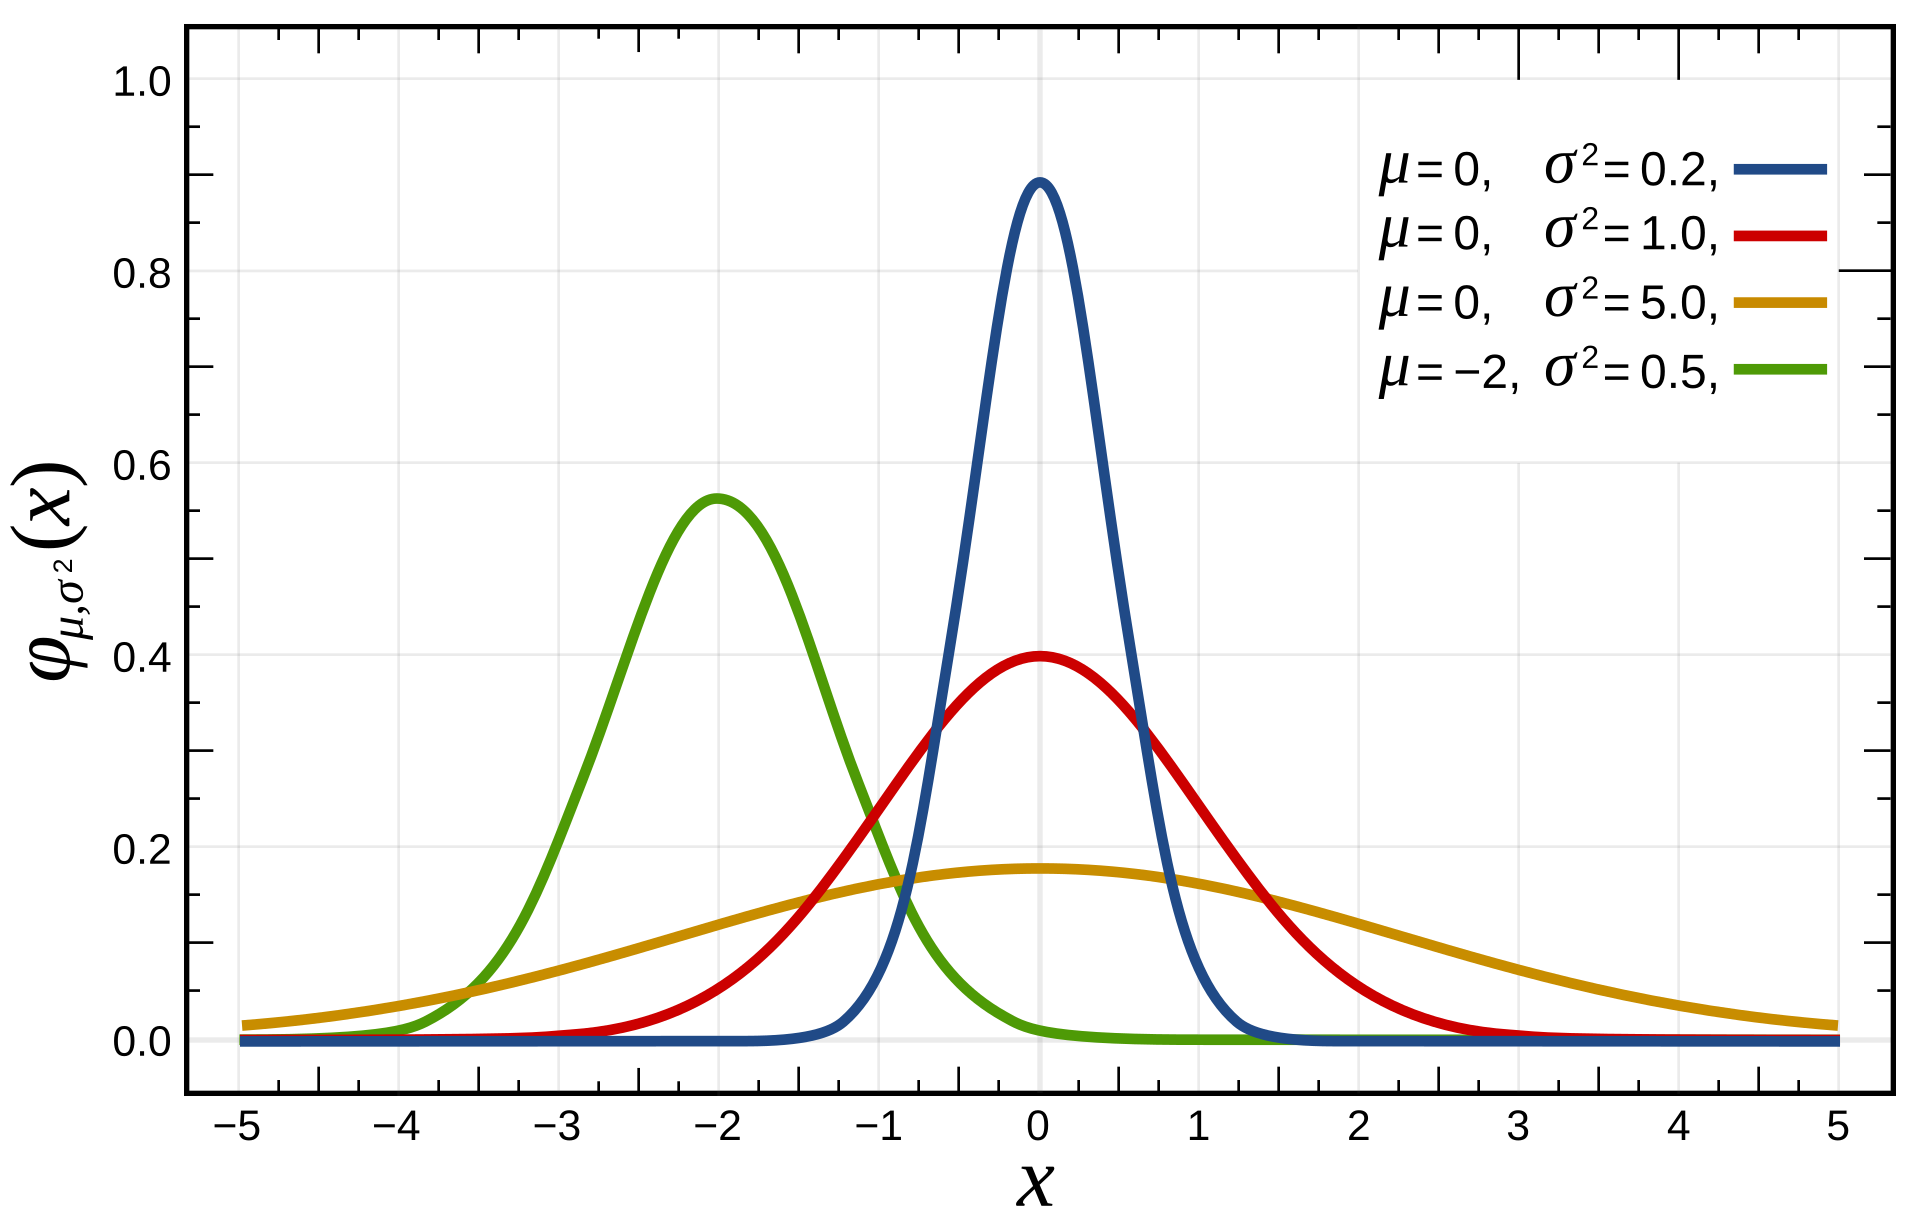
\includegraphics[width=0.45\linewidth]{pics/1d_density.png}
    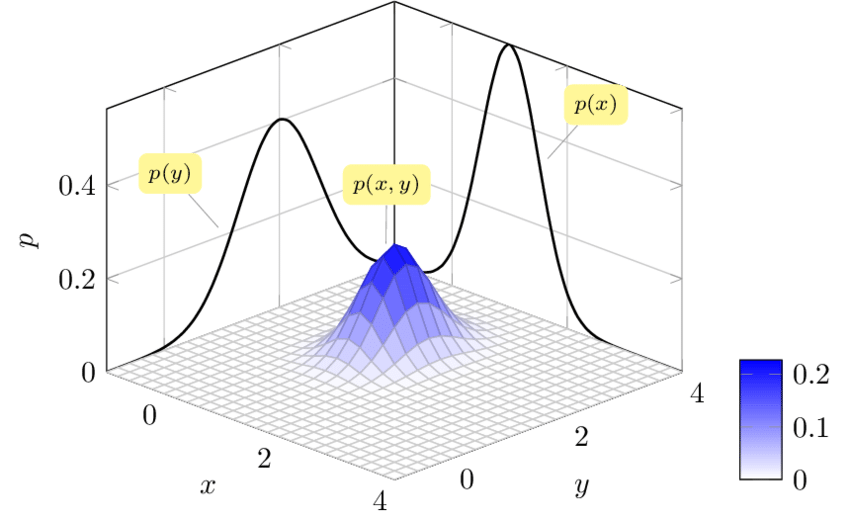
\includegraphics[width=0.45\linewidth]{pics/2d_density.png}
    \caption{Visualization of 1d and 2d Gaussian densities}
    \label{fig:densities_visualization}
\end{figure}

Clearly, the following properties hold
\begin{align}
    \forall x \in \Omega\,,\; p(x) \geq 0\,\; \text{ and }\; \int_\Omega dx\; p(x) = P(\Omega) = 1\,.
\end{align}
Note that this follows from the definition of the random variable.
However, quite often people see some non-negative function $f(x) \geq 0$, and they prove that $\int_\Omega dx\; f(x) < \infty$, i.e. the function is normalizable. 
Then they jump to defining the corresponding probability density function as
\begin{align}
    p(x) = \frac{f(x)}{\int_\Omega dx\; f(x)}\,,
\end{align}
because if the function $f(x)$ is good enough it is true, and because it is useful in practice \kir{which is the whole point of the Monte Carlo methods}.

\begin{example}
    Consider $f(x) = \exp\left(-\frac{1}{2}x^2\right)$, find the corresponding density by finding the normalization constant $\int_{\mathbb{R}} dx\; f(x)$.
\end{example}
\begin{proof}
Let's denote
\begin{align}
    Z \coloneqq \int_{\mathbb{R}} dx\;\exp\left(-\frac{1}{2}x^2\right)\,,
\end{align}
then we have
\begin{align}
     Z^2 = \int_{\mathbb{R}^2} dxdy\;\exp\left(-\frac{1}{2}(x^2+y^2)\right)\,.
\end{align}
Taking $x = r\cos \phi\,, y = r\sin \phi$, we have
\begin{align}
    Z^2 = \int_0^{2\pi}d\phi\;\int_0^\infty dr\;\exp\left(-\frac{1}{2}r^2\right)r = 2\pi \int_0^\infty dy\;\exp\left(-y\right) = 2\pi\,.
\end{align}
Thus, we have
\begin{align}
    p(x) = \frac{1}{\sqrt{2\pi}}\exp\left(-\frac{1}{2}x^2\right)\,.
\end{align}
\end{proof}

\begin{mybox}
\begin{definition}[Normal distribution]\label{def:normal_pdf}
    The density of the Normal distribution or Gaussian distribution is given by the following formula
    \begin{align}
        \Normal(x\cond \mu, \sigma^2) = \frac{1}{\sqrt{2\pi\sigma^2}}\exp\left(-\frac{1}{2\sigma^2}(x-\mu)^2\right)\,.
    \end{align}
    For $\mu=0,\sigma=1$, we call it the \textit{standard} normal distribution.
\end{definition}
\end{mybox}

\subsection{Joint, Marginal, Conditional distributions}

Consider two random variables $X,Y$ that we observe together.
The joint distribution of these random variables is another random variable, which space of outcomes and the corresponding sigma-algebra can be formally constructed using \cref{def:rv}.

\begin{mybox}
\begin{definition}[Joint distribution]\label{def:joint_dist}
    Consider two random variables $X$ with $(\Omega_x, \mathcal{F}_x, P_x)$ and $Y$ with $(\Omega_y, \mathcal{F}_y, P_y)$, then we can define
    \begin{enumerate}
        \item $\Omega = \Omega_x \times \Omega_y$, i.e. the joint outcome space is the direct product of the outcome spaces.
        \item $\mathcal{F} = \mathcal{F}_x \times \mathcal{F}_y$, the product of sigma-algebras can be constructed as the minimal sigma-algebra that contains the set $\{(A_1, A_2): A_1 \in \mathcal{F}_x\,,\; A_2 \in \mathcal{F}_y\}$.
        \item $P: \mathcal{F} \to [0,1]$, and, importantly, it cannot be defined simply through the knowledge of $X$ and $Y$. We have to define this probability measure from other principles, e.g. the observations that we collected by observing $X$ and $Y$ simultaneously.
    \end{enumerate}
\end{definition}
\end{mybox}
Once again, this definition is something that tells us that we have the right to reason about these things, but doesn't give us the tools to reason.

In practice, we usually start from the joint probability or the joint density because it contains the full information about all the random variables involved.
That is, for the discrete variables $\{X_i\}_{i=1}^n$ taking values $x_i$ in integer numbers $\mathbb{Z}$, the joint probability is usually defined as a function that maps integers to probability values, i.e.
\begin{align}
    P: \mathbb{Z}^n \to [0,1]\,, \text{ and for the value at given point we write } P(X_1 = x_1, \ldots, X_n = x_n) = P(x_1, \ldots, x_n)\,.
\end{align}
For the continuous random variables, we define the joint distribution through the joint density. 
That is, for the random variables $\{X_i\}_{i=1}^n$ taking values $x_i$ in the Euclidean space $\mathbb{R}^m$ (not necessarily of the same dimension), we have the density function $p$ that evaluates probabilities
\begin{align}
    \int_A dx\; p(x) = P(X \in A)\,,
\end{align}
where $A$ is in the joint sigma-algebra, $X$ is the joint outcome and $P$ is defined as the probability measure on the joint sigma-algebra.
Clearly, the following holds for the density function
\begin{align}
    p(x_1,\ldots, x_n) \geq 0\,, \;\; \int_{\mathbb{R}^{mn}} dx_1\ldots dx_n\; p(x_1,\ldots,x_n) = 1\,.
\end{align}
Note that there is not much difference between what we considered for the single random variable.
All the differences are hidden in the way we construct the Kolmogorov triplet.

Interesting differences appear when we start ``disassembling'' the joint distribution back into individual random variables and study relations between these variables.
Consider the following function
\begin{align}
    F(x) \coloneqq \sum_{y \in \mathbb{Z}} P(X = x, Y = y)\,,
\end{align}
where $P(X = x, Y = y)$ is the probability function of random variables $X$ and $Y$ and we sum over all possible values of $Y$.
Note that we are summing over disjoint outcomes \kir{indeed, we can't observe $Y$ to take two different values and our outcome space is the product of outcome spaces of $X,Y$}.
We can rewrite it as follows
\begin{align}
    F(x) \coloneqq \sum_{y \in \mathbb{Z}} P(X = x, Y = y) = P(\cup_{y \in \mathbb{Z}} (X = x, Y = y)) = P((X = x, Y \in \Omega_y)) = P(X = x)\,,
\end{align}
where in the last transition we drop the dependency on $Y$ since it always holds.
This motivates the following definition.

\begin{mybox}
\begin{definition}[Marginal distribution]\label{def:marg_dist}
    For the discrete random variables $X,Y$, the marginal distributions of $X$ and $Y$ are defined as follows
    \begin{align}
        P(x) \coloneqq \sum_y P(x,y)\,, \; P(y) \coloneqq \sum_x P(x,y)\,.
    \end{align}
    For the continuous random variables $X,Y$, the probability density function of the marginal distribution of $X$ is defined as follows
    \begin{align}
        p(x) \coloneqq \int_{\Omega_y} dy\; p(x,y)\,,\; p(y) \coloneqq \int_{\Omega_x} dx\; p(x,y)\,.
    \end{align}
\end{definition}
\end{mybox}

You can think about marginalization as of projection of the joint distribution to one of the ``planes'' corresponding to some random variable. \kir{Nobody stops you from defining a new plane in the joint space and projecting to it}
In the space of observations it corresponds to ``forgetting'' or ``erasing'' the information about $Y$, e.g. if you particles hitting a detector, you can register only one of the coordinates, which corresponds to the marginalization of the joint distribution of coordinates.

In practice, one of the most important concepts is the conditioning.
Intuitively, it corresponds to querying your database with something like "select all the musicians that are 27 years old".
More formally, you can consider all the events $\{(X = i, Y=y)\}_{i \in \mathbb{Z}}$, i.e. we fix the value of $Y$ at $y$ and make a collection of all such events by varying $X$.
Note that clearly $P(X = i, Y = y) \geq 0$ for all $i$, hence it is almost a valid probability function, the only problem is that it doesn't normalize to $1$, i.e.
\begin{align}
    \sum_{i\in \mathbb{Z}} P(X = i, Y = y) < 1\,,
\end{align}
because $y$ is fixed and we can't sum over all events in the joint outcome space $\Omega$.
This function, though, makes total sense, and we can think about events of the type ``$X < 0$ and $Y = 6$''.
The solution to this problem is to define a new random variable that corresponds to the ``slice'' of the entire outcome space where $Y = y$.
This leads to the following \textit{definition}!

\begin{mybox}
\begin{definition}[Conditional distribution]\label{def:cond_dist}
    For the discrete random variables $X,Y$, the conditional distribution of $X$ for $Y = y$ is defined as
    \begin{align}
        P(X = x\cond Y = y) \coloneqq \frac{P(X = x, Y = y)}{P(Y = y)}\,.
    \end{align}
    For the continuous random variables $X,Y$, the probability density function of the conditional distribution of $X$ for $Y = y$ is defined as
    \begin{align}
        p(x\cond y) \coloneqq \frac{p(x,y)}{p(y)}\,.
    \end{align}
\end{definition}
\end{mybox}
The vertical line in the notation separates the random variables from the conditions.
In other words, $p(x\cond y)$ defines a random variable on $X$ but not on $y$, this is easy to see by evaluating the normalization constants of the conditional distribution.

\begin{corollary}[Normalization of conditional distribution]
    Conditional distribution normalizes to $1$, i.e. defines a valid random variable.
\end{corollary}
\begin{proof}
    By the straightforward accounting exercises, we have
    \begin{align}
        \sum_x P(x\cond y) = \sum_x \frac{P(x,y)}{P(y)} = \frac{1}{P(y)}\sum_x P(x,y) = \frac{1}{P(y)}P(y) = 1\,,
    \end{align}
    and
    \begin{align}
        \int dx\; p(x\cond y) = \frac{1}{p(y)}\int dx\; p(x,y) = \frac{1}{p(y)}p(y) = 1\,.
    \end{align}
\end{proof}
\kir{note that a lot of results translate seamlessly from the discrete case to the continuous (which i have been abusing above by reasoning in the discrete case and then applying for the continuous). This is not always the case, but we can't keep writing everything for both cases all the time. There is no default choice, or a ``better'' choice, the answer might be disappointing for you, but you have to know both and to know all the bridges between both. Thus, by making progress in one of the worlds you can jump to another and get some insights there.}

Note that for different $y$, according to \cref{def:cond_dist}, we have different distributions $p(x\cond y)$.
However, what if it is not the case?
In other words, consider the special case when
\begin{align}
    p(x\cond y) = p(x)\,,\; \forall y.
\end{align}
Then it makes sense to call random variables $X$ and $Y$ independent, because the distribution of $X$ is not anyhow affected by our choice of $y$.
Using \cref{def:cond_dist}, we have
\begin{align}
    \frac{p(x,y)}{p(y)} = p(x)\,, \implies p(x,y) = p(x)p(y)\,.
\end{align}

\begin{mybox}
\begin{definition}[Independent random variables]\label{def:independent_rvs}
    Two random variables $X,Y$ are called independent if their joint pdf is a product of the marginal pdfs, i.e.
    \begin{align}
        p(x,y) = p(x)p(y)\,.
    \end{align}
\end{definition}
\end{mybox}
\kir{Please note that this is not some philosophical definition of independence and you can make some conclusions based on this. 
This is the mathematical definition that means exactly what is written. See example below} 
\begin{example}
    Consider a king on a chess board going forward and backward as shown in \cref{fig:chess_king}. After a big number of steps, the distribution of $X$ and $Y$ coordinates of its position is going to be uniform. However, it doesn't mean that we can't predict where the king will move next.
\end{example}
\begin{figure}[t]
    \centering
    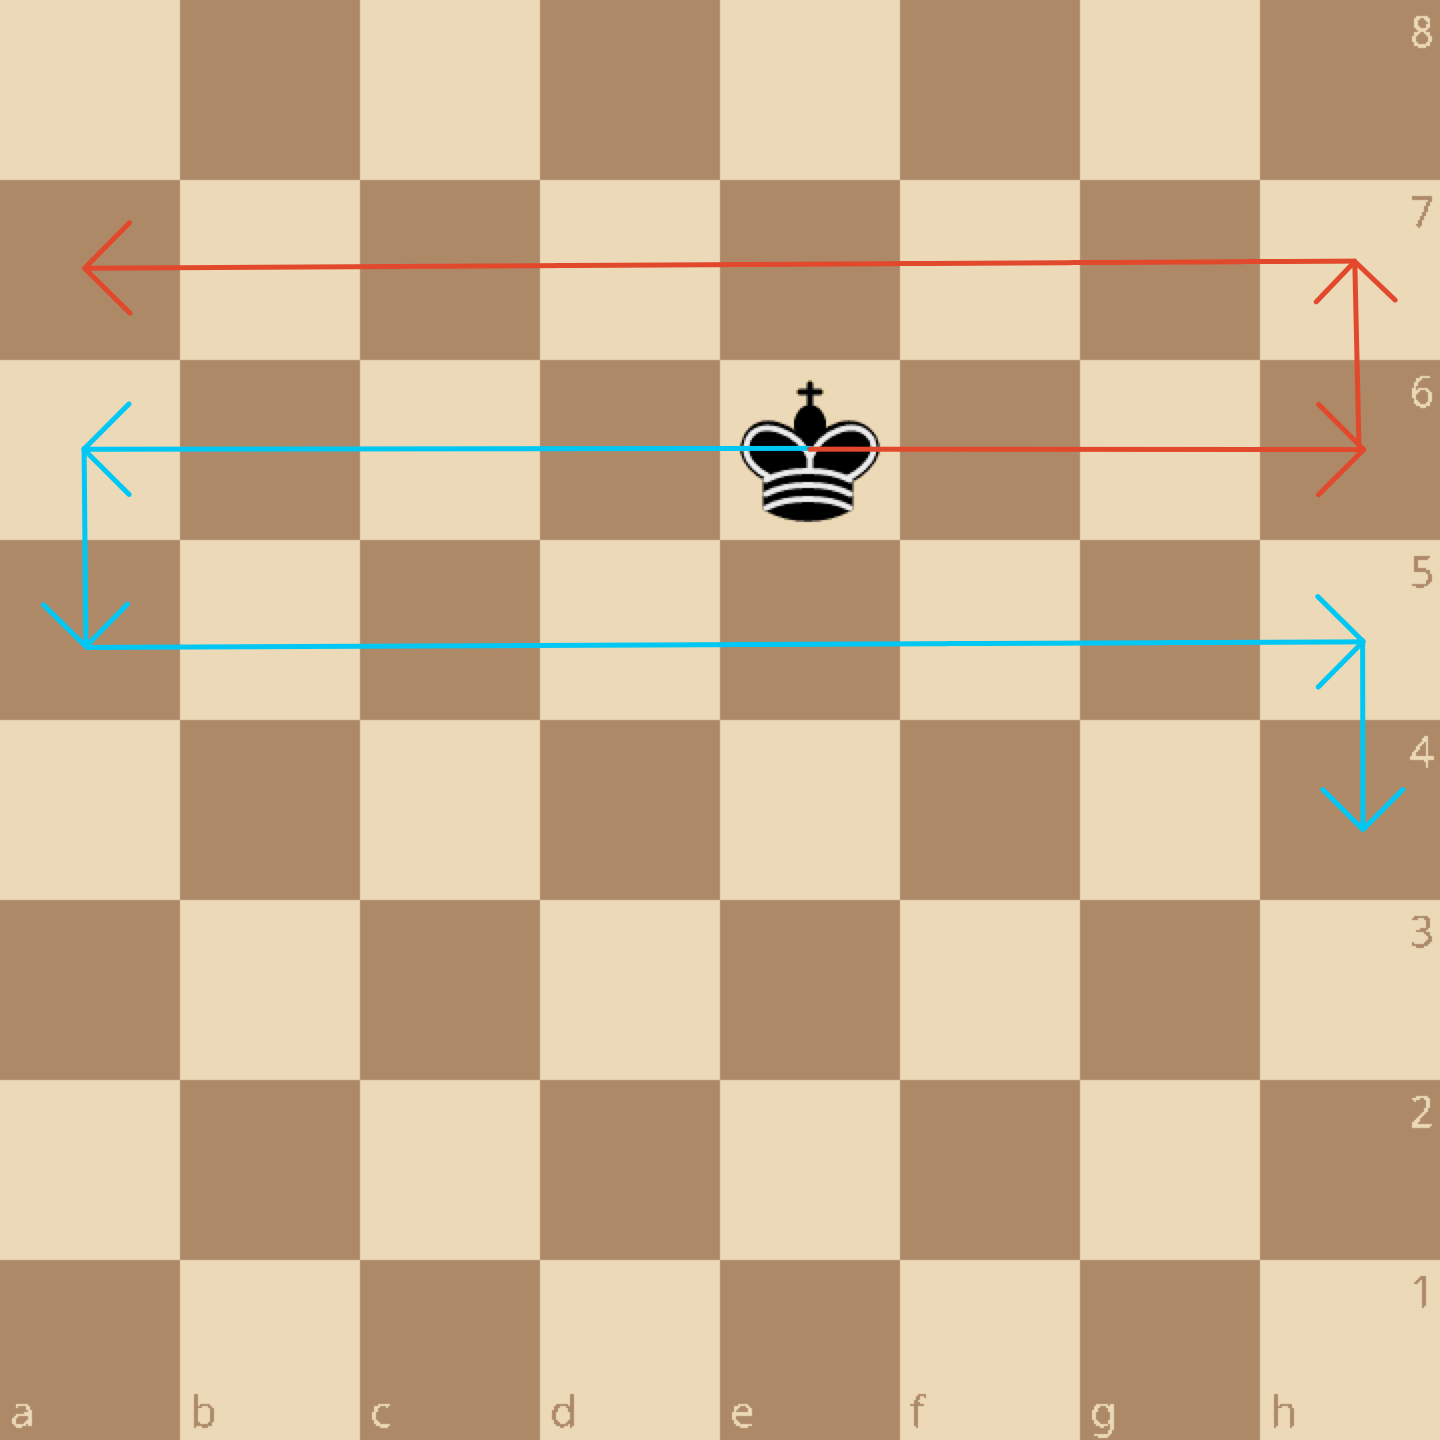
\includegraphics[width=0.3\linewidth]{pics/chess_king.png}
    \caption{Example of the process that generates independent distributions (horizontal and vertical coordinates of the king) but is completely deterministic and predictable}
    \label{fig:chess_king}
\end{figure}

In theory, everything looks symmetric and there is no conceptual difference between $p(x\cond y)$ and $p(y\cond x)$.
However, in practice, we usually know only one of these conditional probabilities and we would like to find the other.

Let's say we know the distribution of $X$ through density $p(x)$ and we know how $Y$ depends on $X$, i.e. we know $p(y\cond x)$.
Oftentimes we are interested in ``inverting the function'' $p(y\cond x)$, i.e. in finding $p(x\cond y)$ \kir{sometimes finding the posterior distribution is called the inverse problem}.
This can be done as follows
\begin{align}
    p(x\cond y) = \frac{p(x,y)}{p(y)} = \frac{p(x,y)}{\int_{\Omega_x} dx\; p(x,y)} = \frac{p(y \cond x)p(x)}{\int_{\Omega_x} dx\; p(y \cond x)p(x)}\,,
\end{align}
where we used the definitions of marginal and conditional distributions.
People refer to this result as Bayes' theorem, as follows.
\begin{theorem}[Bayes' theorem]
\label{th:bayes}
    Conditional density $p(x\cond y)$ can be written using the conditional density $p(y\cond x)$ and the marginal density $p(x)$ as follows
    \begin{align}
        p(x\cond y) = \frac{p(y\cond x)p(x)}{\int_{\Omega_x} dx\; p(y\cond x)p(x)}\,.
    \end{align}
\end{theorem}
This course is devoted to different practical solutions of probabilistic inverse problems based on this result.

\begin{exercise}[Medical Tests]
    Consider the test $t$ for some disease $d$, which conditional distribution $p(t\cond d)$ is defined in the table below. Assuming that we know the marginal distribution of $d$ ($p(d=1) = 0.5$) for the disease, find $p(d = 1\cond t = 1)$
    \begin{center}
    \begin{tabular}{c|cc}
         & $p(t = 1\cond d)$ & $p(t = 1\cond d)$  \\
        \midrule
        d=1 & 0.99 & 0.01 \\
        d=0 & 0.01 & 0.99
    \end{tabular}
    \end{center}
    How the result changes if the disease is very rare ($p(d=1) = 10^{-4}$)?
\end{exercise}

\begin{example}
    Consider the discrete distribution $P(Y = 0) = P(Y = 1) = 1/2$ and the continuous distribution $X\cond Y$ which has the density $\Normal(x\cond y, \sigma^2)$.
    Using the Bayes' theorem, we have
    \begin{align}
        P(Y = 1 \cond x) =~& \frac{p(x\cond y= 1)P(Y=1)}{p(x\cond y= 0)P(Y=0) + p(x\cond y= 1)P(Y=1)}\\
        =~& \frac{\Normal(x\cond 1,\sigma^2)}{\Normal(x\cond 0,\sigma^2) + \Normal(x\cond 1,\sigma^2)} = \frac{\exp\left(-\frac{1}{2\sigma^2}(x-1)^2\right)}{\exp\left(-\frac{1}{2\sigma^2}(x-1)^2\right) + \exp\left(-\frac{1}{2\sigma^2}x^2\right)} \\
        =~& \frac{1}{1 + \exp\left(-\frac{1}{2\sigma^2}\left[x^2 - x^2 +2x - 1\right]\right)} = \frac{1}{1 + \exp\left(-\frac{1}{2\sigma^2}\left[2x - 1\right]\right)}
    \end{align}
    The resulting probability depends on $x$ and is described by the sigmoid function (see \cref{fig:sigmoids})
\end{example}

\begin{figure}[t]
    \centering
    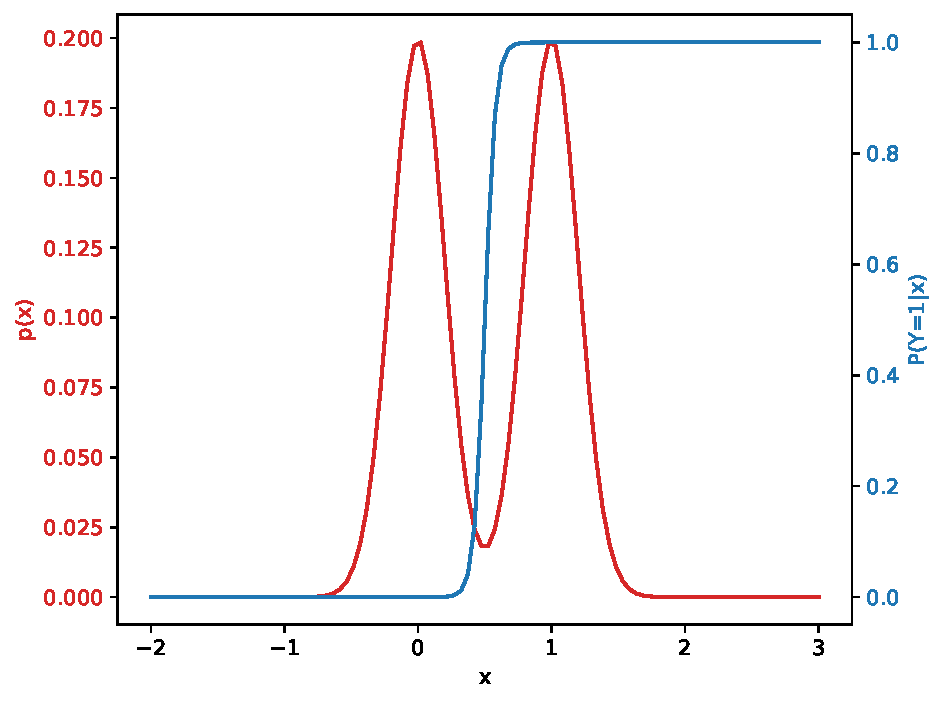
\includegraphics[width=0.45\linewidth]{pics/sigmoid_sharp.pdf}
    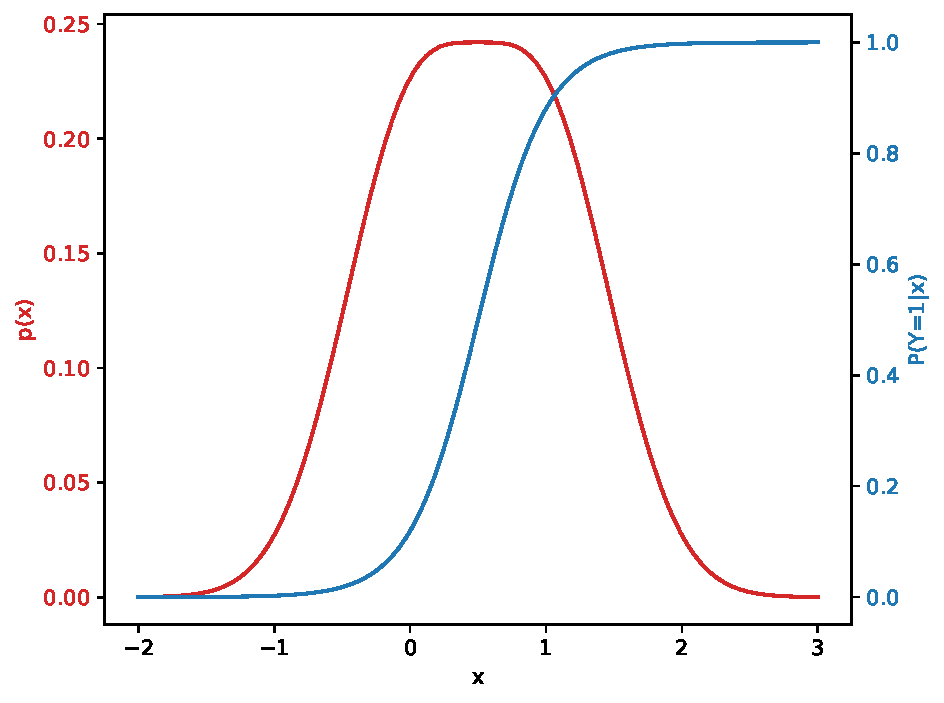
\includegraphics[width=0.45\linewidth]{pics/sigmoid_mix.pdf}
    \caption{Density $p(x)$ and the probability $P(Y=1\cond x)$ for $\sigma=0.2$ (left) and $\sigma=0.5$ (right).}
    \label{fig:sigmoids}
\end{figure}

\begin{mybox}
\begin{definition}[Bernoulli random variable]\label{def:bern_rv}
    The random variable $X$ defined on two states $\Omega = \{0,1\}$ \kir{the states can be anything, ofc} defines the Bernoulli random variable, i.e.
    \begin{align}
        X = \begin{cases}
            1\,, \; \text{ with prob. } \; \theta\,,\\
            0\,, \; \text{ with prob. } \; (1-\theta)\,,
        \end{cases}
        \label{eq:bernoulli_def}
    \end{align}
    where $\theta \in [0,1]$ is a parameter. For $\theta=1/2$, some people call this random variable "fair coin".
\end{definition}
\end{mybox}

Oftentimes, we have a number of \textit{independent} Bernoulli random variables and we want to reason about how many of them equal $1$ and how many of them equal $0$.
First, we will rewrite the probability function of a single Bernoulli variable as follows
\begin{align}
    P(x\cond \theta) = \theta^x (1-\theta)^{1-x}\,,
\end{align}
which, as you can see, corresponds to \cref{eq:bernoulli_def}.
However, now we can multiply this probability functions according to \cref{def:independent_rvs}, i.e.
\begin{align}
    P(x_1,\ldots,x_n\cond \theta) = \theta^{\sum_i x_i} (1-\theta)^{\sum_i (1-x_i)}\,,
\end{align}
which serves as a motivation to another random variable in the following definition.

\begin{mybox}
\begin{definition}[Binomial random variable]\label{def:binomial_rv}
    Consider $n$ \textit{independent} Bernoulli random variables with the parameter $\theta$. The Binomial random variable $X$ is defined as the \textbf{number} of Bernoulli variables that are equal $1$, i.e.
    \begin{align}
        P(X = k \cond \theta, n) = C_n^k \theta^k (1-\theta)^{n-k}\,.
    \end{align}
\end{definition}
\end{mybox}

\begin{exercise}
    Prove the formula from \cref{def:binomial_rv}.
\end{exercise}

\begin{mybox}
\begin{definition}[Poisson random variable]\label{def:poisson_rv}
    Poisson random variable $X$ with the rate $\lambda$ is defined as
    \begin{align}
        P(X = k\cond \lambda) = \exp(-\lambda)\frac{\lambda^k}{k!}.
    \end{align}
    \kir{usually the Poisson random variable defines some sequence of events happening randomly in time (e.g., earthquakes) that's why it makes sense to call its parameter the ``rate''.}
\end{definition}
\end{mybox}
\begin{exercise}
    Prove additivity of the Poisson random variables, i.e. for $X_1 \sim \text{Poiss}(\lambda_1)$ and $X_2 \sim \text{Poiss}(\lambda_2)$, prove that $X_1 + X_2 \sim \text{Poiss}(\lambda_1+\lambda_2)$.
\end{exercise}

\subsection{Probabilistic Graphical model}

We can always reason about all the present random variables by writing the joint distribution of all of them.
However, oftentimes, there is a lot of structure in the dependencies (according to \cref{def:independent_rvs}) between the variables.
It is very convenient to depict the relations between the variables graphically, that's why the community has agreed on the following definition.

\begin{mybox}
\begin{definition}[Probabilistic Graphical model]\label{def:graph_model}
    \textit{Acyclic directed graph} is defines a probabilistic graphical model in the following way
    \begin{align}
        p(x_1,\ldots,x_n) = \prod_{i=1}^n p(x_i \cond \texttt{parents of } x_i)\,.
    \end{align}
\end{definition}
\end{mybox}
For instance, the graph in \cref{fig:graphical_model} defines the following joint distribution
\begin{align}
    p(H,P,E,D,T) = p(T\cond E) p (E\cond P,D) p(H \cond P)p(P)p(D).
\end{align}

\begin{exercise}
    Draw the probabilistic graphical model for the Markov chain probabilistic model
    \begin{align}
        p(x_1,\ldots,x_n) = p(x_0)\prod_{i=0}^{n-1}p(x_{i+1}\cond x_i)\,,
    \end{align}
    for the auto-regressive probabilistic model
    \begin{align}
        p(x_1,\ldots,x_n) = p(x_0)\prod_{i=0}^{n-1}p(x_{i+1}\cond x_i,x_{i-1}\ldots, x_0)\,.
    \end{align}
\end{exercise}

\begin{exercise}
\label{exs:graph_model}
    The model consists of the following random variables: the student went to a party $P \in \{0,1\}$, the student has a depression $D \in \{0,1\}$, the student has a headache $H \in \{0,1\}$, results of the exam are good $E \in \{0,1\}$, the teacher is happy $T \in \{0,1\}$. The relations between these variables are given in \cref{fig:graphical_model} and the conditional probabilities are defined as follows
    \begin{center}
    \begin{tabular}{cc|c}
        $P$ & $D$ & $P(E = 0\cond P,D)$  \\
        \midrule
        $1$ & $1$ & $0.999$ \\
        $0$ & $1$ & $0.9$ \\
        $1$ & $0$ & $0.9$ \\
        $0$ & $0$ & $0.01$
    \end{tabular}
    \begin{tabular}{c|c}
        $P$ & $P(H = 1\cond P)$  \\
        \midrule
        $1$ & $0.999$ \\
        $0$ & $0.9$ \\
        & \\
        & \\
    \end{tabular}
    \begin{tabular}{c|c}
        $E$ & $P(T = 1\cond E)$  \\
        \midrule
        $1$ & $0.5$ \\
        $0$ & $0.95$ \\
        & \\
        & \\
    \end{tabular}
    \begin{tabular}{c}
        $P(P = 1) = 0.2$\\
        $P(D = 1) = 0.4$.
    \end{tabular}
    \end{center}
    Find the following probabilities $P(P=1\cond H=1)$, $P(P=1\cond T=0)$, $P(P=1\cond T=0, H=1)$.
\end{exercise}

\begin{figure}[t]
    \centering
    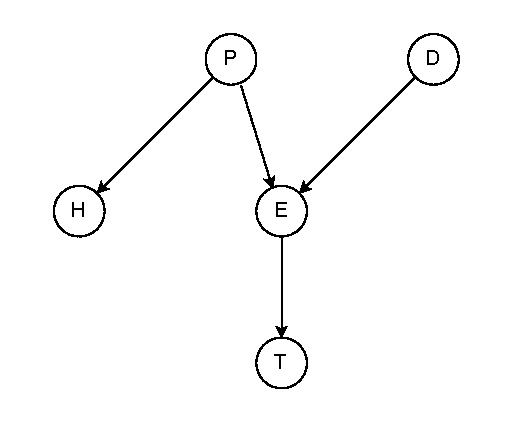
\includegraphics[width=0.4\linewidth]{pics/graphical_model.pdf}
    \caption{Probabilistic graphical model for \cref{exs:graph_model}.}
    \label{fig:graphical_model}
\end{figure}

\subsection{Maximum Likelihood}

In practice, we don't usually know the probabilistic model of some phenomenon, and we would like to design such a model.
The design process of a probabilistic model consists of two main stages:
\begin{enumerate}
    \item Choosing the parametric family of the probabilistic model, i.e. defining how exactly the density value (or probability) $p(x\cond \theta)$ depends on the parameters $\theta$.
    \item Estimating the parameters $\theta$ from the given dataset of observations $\{x_1,\ldots, x_N\}$.
\end{enumerate}

Let's assume that we know exactly the parametric family $p(x\cond \theta)$, i.e. we know for sure that the data we are modeling was generated according to this distribution.
Then one can use the maximum likelihood principle to estimate the parameters $\theta$ from the data.

\begin{mybox}
\begin{definition}[Maximum likelihood]
\label{def:mle}
    For the given parametric family $p(x\cond \theta)$, and the empirical data $\{x_1,\ldots, x_N\}$, Maximum Likelihood Estimator (MLE) of parameters $\theta \in \Theta$ is defined as
    \begin{align}
        \theta_{\text{MLE}} = \argmax_{\theta \in \Theta} p(\{x_1,\ldots, x_N\}\cond \theta)\,,
    \end{align}
    where the density (or probability) $p(\{x_1,\ldots, x_N\}\cond \theta)$ is called likelihood.
\end{definition}
\end{mybox}
If the data was acquired through repeating the same experiment over and over again with the same conditions, it is reasonable to assume \kir{this is a very big and crucial assumption for statistics and machine learning} that the observations $\{x_1,\ldots, x_N\}$ are iid, i.e.
\begin{align}
    p(\{x_1,\ldots, x_N\}\cond \theta) = \prod_{i=1}^N p(x_i\cond \theta)\,.
\end{align}
Under this assumption it's convenient to introduce the following definition.
\begin{mybox}
\begin{definition}[Log-likelihood]\label{def:ll}
    For the given parametric family $p(x\cond \theta)$, and the iid samples $\{x_1,\ldots, x_N\}$, log-likelihood is defined as
    \begin{align}
        \ell(\theta) = \log p(\{x_1,\ldots, x_N\}\cond \theta) = \log \prod_{i=1}^N p(x_i\cond \theta) = \sum_{i=1}^N\log p(x_i\cond \theta)\,.
    \end{align}    
\end{definition}    
\end{mybox}

The maximum likelihood estimator yields closed-form solution for many parametric distribution just by writing down the necessary conditions for the maximum.
\begin{example}[MLE for the Binomial distribution]
    Consider $\mathcal{D}= \{x_1,\ldots,x_N\}$ --- iid samples from the Binomial distribution $\text{Binom}(x\cond n, \theta)$. 
    The log-likelihood for $\theta$ is
    \begin{align}
        \ell(\theta) = \sum_{i=1}^N \log \left(C_{n}^{x_i}\theta^{x_i}(1-\theta)^{n-x_i}\right) = \sum_{i=1}^N  \left(\log C_{n}^{x_i} + x_i\log \theta + (n-x_i)\log(1-\theta)\right)\,.
    \end{align}
    From the maximum likelihood principle, we have
    \begin{align}
        0 =~& \deriv{}{\theta}\ell(\theta) = \sum_{i=1}^N  \left(x_i\frac{1}{\theta} + (n-x_i)\frac{1}{1-\theta}\right)\,,\\
        (1-\theta)\sum_i x_i =~& \theta\sum_i(n-x_i)\\
        \theta_{\text{MLE}} =~& \frac{\sum_i x_i}{\sum_i n} = \frac{1}{N}\sum_i \frac{x_i}{n}\,.
    \end{align}
    It is the average success rate over all the experiments.
\end{example}

The following theorem is one of the main motivations for using MLE.
\begin{theorem}[Convergence of MLE]
    Consider the set of iid samples $\mathcal{D} = \{x_1,\ldots, x_N\}$ from the categorical distribution $P(x\cond \theta^*)$
    \begin{align}
        P(x = k \cond \theta^*) = \theta^*_k\,,\; \theta^*_k \geq 0\;\forall k\,.
    \end{align}
    The maximum likelihood estimator of $\theta$ (under the ground true probabilistic model) converges (in the number of samples) to the ground true parameters, i.e.
    \begin{align}
        \lim_{N\to\infty} \theta_{\text{MLE}} = \theta^*\,.
    \end{align}
\end{theorem}
\begin{proof}
    The log-likelihood of the dataset is
    \begin{align}
        \ell(\theta) =~& \frac{1}{N}\sum_{i=1}^N\log P(x_i\cond \theta) = \frac{1}{N}\sum_{k=1}^MN_k\log P(x_i=k\cond \theta)\\
        =~& \frac{1}{N}\sum_{k=1}^MN_k\log \theta_k = \sum_{k=1}^M\frac{N_k}{N}\log \theta_k\,,
    \end{align}
    where $N_k$ is the number of samples that equal $k$, i.e. $N_k = |\{x \in \mathcal{D}  \cond x = k\}|$.
    From the maximum likelihood principle, we have
    \begin{align}
        \theta_{\text{MLE}} = \argmax \ell(\theta)\,, \;\text{ s.t. }\; \sum_{k=1}^M\theta_k = 1\,,\; \theta_k \geq 0\;\forall k\,.
    \end{align}
    The corresponding Largangian is
    \begin{align}
        \mathcal{L}(\theta) = \ell(\theta) + \lambda \sum_{k=1}^M(\theta_k - 1)\,,
    \end{align}
    and the necessary condition for the optimum is
    \begin{align}
        \forall k\,,\;0 = \deriv{\ell(\theta)}{\theta_k}  + \lambda = \frac{1}{\theta_k}\frac{N_k}{N}  + \lambda \implies \theta_k = \frac{N_k}{N}\,.
    \end{align}
    Thus, we have
    \begin{align}
        \theta_{\text{MLE}} = \begin{bmatrix}
            \ldots\\
            \frac{N_k}{N}\\
            \ldots
        \end{bmatrix}\,.
    \end{align}
    For the limit of the infinite number of samples, we have
    \begin{align}
        \lim_{N\to\infty} (\theta_{\text{MLE}})_k = \lim_{N\to\infty}\frac{N_k}{N} = P(X=k\cond \theta^*) = \theta^*_k\,.
    \end{align}
\end{proof}
Thus, we have demonstrated that if we know the probabilistic model $p(x\cond\theta)$ exactly, then for any given precision of the parameter estimation $\theta$ we can collect the dataset $\mathcal{D}$ large enough to satisfy this precision.

\begin{exercise}
    Consider $x_1,\ldots,x_N$ --- iid samples from the Normal distribution $\mathcal{N}(x\cond \mu, \sigma)$. Find the maximum likelihood estimation of $\mu,\sigma$.
\end{exercise}

\begin{exercise}
    Consider $x_1,\ldots,x_N$ --- iid samples from the Poisson distribution $\text{Poiss}(\lambda)$. Find the maximum likelihood estimation of $\lambda$.
\end{exercise}

\begin{proposition}[MLE for regression]
    Consider the dataset $\mathcal{D} = \{(x_i, y_i)\}_{i=1}^N$, where $x \in \mathbb{R}^d$ and $y \in \mathbb{R}$.
    Assuming the following probabilistic model for the dataset
    \begin{align}
        y = f(x;\theta) + \eps\,, \eps \sim \Normal(\eps\cond 0,\sigma^2)\,,
    \end{align}
    where $f$ is some known function.
    find the maximum likelihood estimation of $\theta$ and $\sigma$
\end{proposition}
\begin{proof}
    First, let's rewrite the probabilistic model in a more familiar form
    \begin{align}
        p(y\cond x,\theta,\sigma) = \Normal(y\cond f(x;\theta), \sigma^2)\,.
    \end{align}
    Note that here $y$ is conditioned on the features $x$, parameters of the mean predictor $\theta$ and the standard deviation $\sigma$.
    The log-likelihood of this probabilistic model is
    \begin{align}
        \ell(\theta,\sigma) = \frac{1}{N}\sum_{i=1}^N \log \Normal(y_i\cond f(x_i;\theta), \sigma^2) = \frac{1}{N}\sum_{i=1}^N \left[-\frac{1}{2\sigma^2}(y_i-f(x_i;\theta))^2 - \frac{1}{2}\log (2\pi\sigma^2)\right]\,.
    \end{align}
    Hence, we have
    \begin{align}
        \theta_{\text{MLE}} =~& \argmax_\theta \ell(\theta,\sigma) = \argmax_\theta \ell(\theta,\sigma) \frac{1}{N}\sum_{i=1}^N \left[-\frac{1}{2\sigma^2}(y_i-f(x_i;\theta))^2 - \frac{1}{2}\log (2\pi\sigma^2)\right]\\
        =~& \argmin_\theta \frac{1}{N}\sum_{i=1}^N \left[\frac{1}{2\sigma^2}(y_i-f(x_i;\theta))^2\right] = \argmin_\theta \frac{1}{N}\sum_{i=1}^N (y_i-f(x_i;\theta))^2\,.
    \end{align}
    Thus, MLE is equivalent to Mean-Squared Error (MSE) loss function.
    For $\sigma_{\text{MLE}}$, we have
    \begin{align}
        0 = \deriv{\ell(\sigma)}{\sigma} =~& \frac{1}{N}\sum_{i=1}^N \left[\frac{1}{\sigma^3}(y_i-f(x_i;\theta))^2 - \frac{1}{\sigma}\right] = \frac{1}{N}\sum_{i=1}^N \frac{1}{\sigma^3}(y_i-f(x_i;\theta))^2 - \frac{1}{\sigma}\,,\\
        \sigma_{\text{MLE}}^2 = ~& \frac{1}{N}\sum_{i=1}^N (y_i-f(x_i;\theta_\text{MLE}))^2\,.
    \end{align}
    Thus, the MLE for $\sigma$ equals the average error that persists for $\theta_{\text{MLE}}$.
\end{proof}

\begin{exercise}
    MLE for Laplace residuals
\end{exercise}

\begin{exercise}
    MLE for logistic regression
\end{exercise}

